\section{Comparison of NLP Transformer Models}
\label{sxn:nlp}

[THESE RESULTS HAVE TO BE REDONE BY REMOVING THE FIRST LAYER...]

In the past two years, nearly 100 open source, pre-trained DNNs for Natural Language Processing (NLP) have emerged,
based on the revolutionary Transformer architecture, including variants of BERT, Transformer-XML, GPT, etc.
The Transformer architectures consist of blocks of Attention layers, containing of 2 large, Feed Forward (Linear)
weight matrics \cite{Attn2017}. In contrast to the smaller pre-Activation maps arising in Cond2D layers,
the Attention matrices are significantly larger, and frequently under-correlated, with generally larger
Heavy Tailed Power Law exponents $\alpha$ (when fitting the ESD).  Here, we breifly look at a few
popular pretrained NLP DNNs to demonstrate that the Theory of Heavy Tailed Self-Regularization also
applies to NLP models and not just CV models, and to highlight how to use the theory to identify
poorly trained models where the empirical norm metrics will perform poorly.

\paragraph{OpenAI GPT Models}
We use the \emph{WeightWatcher} tool to analyze the OpenAI GPT and GPT2 models, which gives us
the opportunity to analyze the effect of both training the same model with different size data sets,
and increasing sizes of both the data set and architectures.
These models have generated significant media attention because of their remarkable ability to
 generate fake text that appears to be real and the potential misuse of this.
For this reason, the original GPT model was trained on on a deficient data set, rendering
the model interesting but not fully functional.  Later, OpenAI released a much improved model--
GPT2 (small)--which has the same architecture and number of layers as GPT, but has
been trained on a larger and better data set (and with other changes), making it
remarkably good at generating (near) human-quality fake text.  
By comparing the poorly trained GPT to the well trained GPT2, we
indentify empirical indidcators for when  model has in fact
been poorly trained and may perform poorly when deployed.

\charles{more here ?}
We analyze GPT models deployed with the popular HuggingFace PyTorch library.
GPT has 12 layers, with 4 Multi-head Attention Blocks, giving $48$ Layer Weight Matrices $\mathbf{W}$.
Each Block has 2 components, the Self Attention (attn) and the Projection (proj) matrics.  
The self-attention  matrices are larger, of dimension ($2304\times 768$) or ($3072\times 768$).
The projection layer concatenates the self-attention results into a vector (of dimension $768$).
This gives $50$ large matrices.

Because GPT and GPT are trained on different data sets, the initial Embedding matrices differ in shape.
GPT  has an initial Token and Positional Embedding layers, of dimension
$(40478\times 768)$ and $(512\times 768)$, resp, whereas GPT2 has input Embeddings of shape
$(50257\times 768)$ and $(1024\times 768)$, resp.  Interstingly, they also have very spectral properties,
also shown below.

The OpenAI GPT2 (English) models are: \nred{gpt-small, gpt-medium, gpt-large, and gpt-xl}, \
having include $12, 24, 36, \text{and }48$ layers, resp., with increasingly larger weight matrices.
The model card for GPT2 is published on github.\footnote{\url{https://github.com/openai/gpt-2/blob/master/model_card.md}}.
Table \ref{table:nlp} reports results for the average log norm metrics, using \emph{weightwatcher (0.2.7)},
and with fully reproducible Jupyter notebooks.\footnote{\url{https://github.com/CalculatedContent/kdd2020}}


\begin{table}[t]
\small
\begin{center}
\begin{tabular}{|p{1in}|c|c|c|c|c|}
\hline
   &    & Frobenius Norm & Spectral Norm & Weighted Alpha & Alpha-Norm \\
 Series & \#Layers   & $\Vert\mathbf{W}\Vert_{F}$ & $\Vert\mathbf{W}\Vert_{\infty}$ & $\hat{\alpha}=\alpha\log\lambda_{max}$ & $\Vert\mathbf{X}\Vert^{\alpha}_{\alpha}$ \\
\hline
GPT & 49 & 1.64  & 1.72 & 7.01 & 7.28 \\
GPT (small) & 49 & 2.04  & 2.54& 9.62 & 9.87 \\
GPT2 medium & 98 & 2.08 & 2.58& 9.74 & 10.01 \\
GPT2 large & 146 & 1.85 & 1.99& 7.67 & 7.94 \\
GPT2 xl & 194 & 1.86 & 1.92 & 7.17 & 7.51 \\
\hline
\end{tabular}
\end{center}
\caption{Average Log Norm Metrics for pretrainnd OpenAI GPT and GPT2 models.}
\label{table:nlp}
\end{table}


\paragraph{The Heavy Tailed Power Law Exponents in GPT and GPT2}

are very differenmt, with GPT2 having both a notably smaller mean $\alpha$, and far fewer, unusually large outliers.
Figure \ref{fig:gpt-alphs-hist} shows the empirical density (histogram) of $\alpha$
for all layers in GPT (blue) and GPT2 (red).  \charles{discuss more}

\begin{figure}
    \centering
    \subfigure[Power Law Exponent $\alpha$]{
        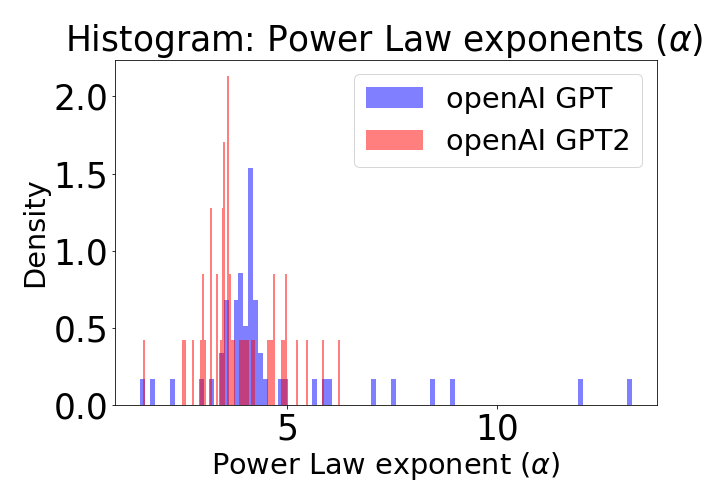
\includegraphics[width=5cm]{img/GPT-alpha-hist.png}
        \label{fig:GPT-alpha.hist.png}
       }
    \qquad
    \subfigure[log Spectral Norm $\log\Vert\mathbf{W}\Vert_{\infty}$]{
        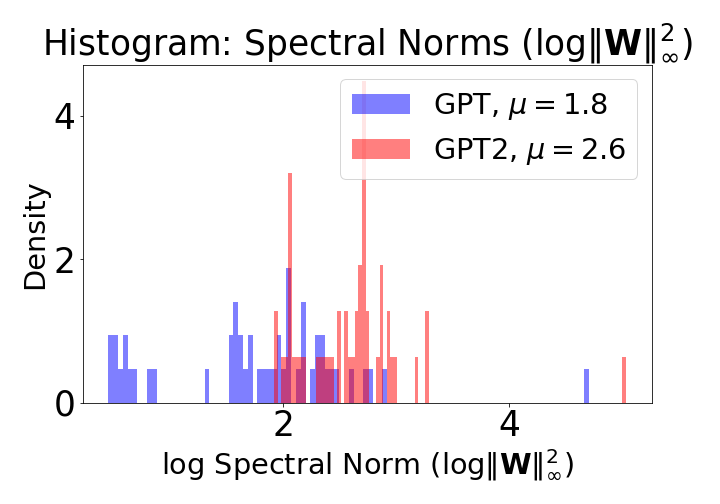
\includegraphics[width=5cm]{img/GPT-snorm-hist.png}
        \label{fig:GPT-snorm.hist.png}
       }


   \caption{Comparison of Heavy Tailed Power Law exponents $\alpha$, and log Spectral Norms $\log\Vert\mathbf{W}\Vert_{\infty}$
for the OpenAI GPT and GPT2 (small) pretrained models.}

\end{figure}

\charles{We have redo the spectral norm and remove the outliers}

\paragraph{The Correlation Flow in GPT and GPT2} also differs significantly between GPT and GPT2.
Figure \ref{fig:gpt-alpha-layer} plots $\alpha$ vs the layer id for each model.


\charles{Discuss Spectral Norm, alpha-Norm}

\begin{figure}[t]
    \centering

    \subfigure[Power Law Exponent $\alpha$]{
        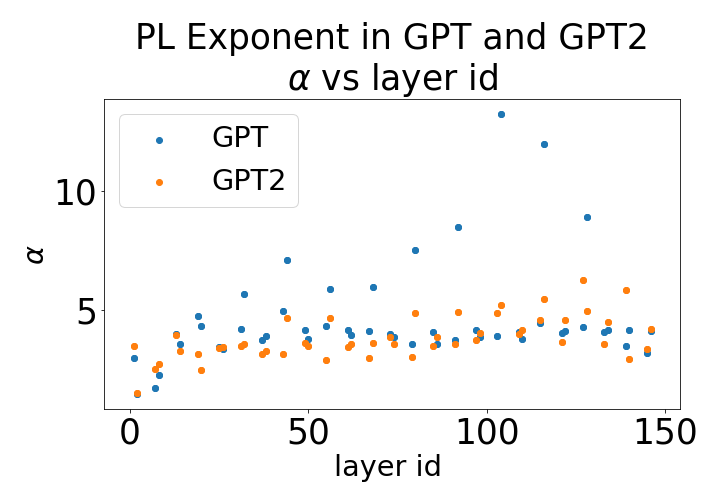
\includegraphics[width=4.5cm]{img/GPT-alpha-depth.png}
        \label{fig:gpt-alpha-layer}
    }
    \qquad
    \subfigure[log Spectral Norm $\log\Vert\mathbf{W}\Vert_{\infty}$]{
        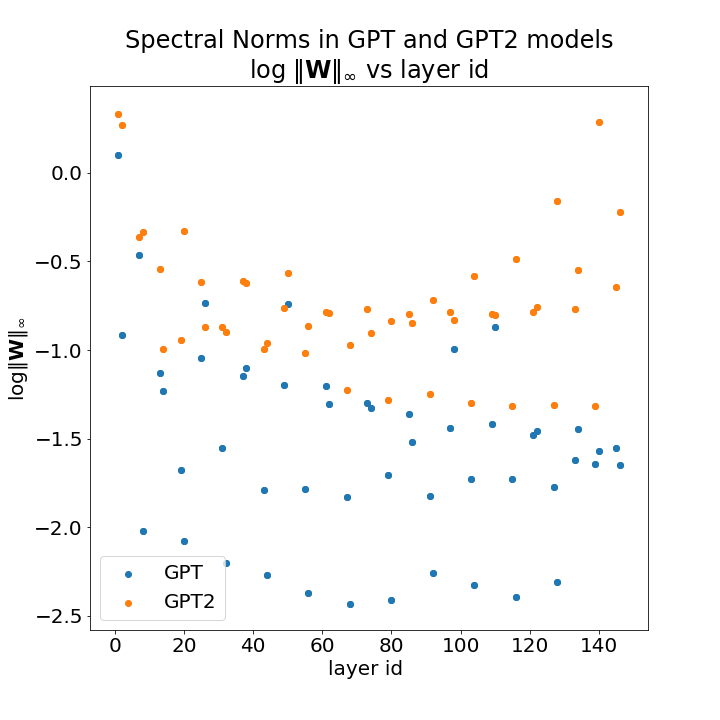
\includegraphics[width=4.5cm]{img/GPT-snorm-depth.png}
        \label{fig:resnet-snorm-layer}
    }
    \qquad
    \subfigure[log Alpha-Norm $\log\Vert\mathbf{X}\Vert_{\alpha}^{\alpha}$]{
        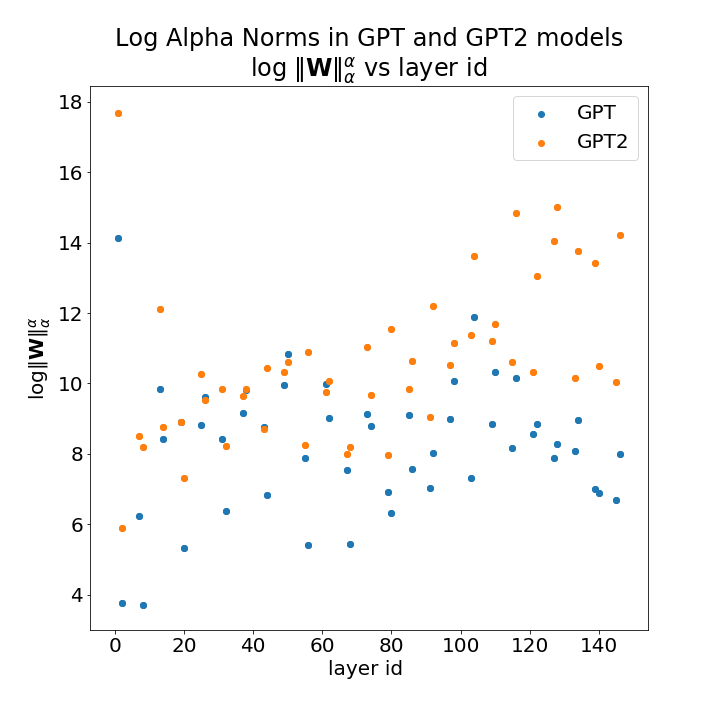
\includegraphics[width=4.5cm]{img/GPT-pnorm-depth.png}
        \label{fig:gpt-pnorm-layer}
    }
    \caption{Comparison of Correlation Flow and Spectral Norm for OpenAI GPT and GPT2   }
    \label{fig:gpt-alpha-layers}
\end{figure}


Notice the first embedding layer(s) have unusually large Spectral Norms,
reflecting a lack of normalization.  For example, in GPT, most layers, the maximum eigenvalue $\lambda_{max}\sim\mathcal{O}(10-100)$,
but in the first embedding layer, the maximum is of order N (the number of words in the embedding), or
 $\lambda_{max}\sim\mathcal{O}(10^{5})$.  For GPT and GPT2, we layer all layers as-is (although one may to normalize
the first 2 layers by  $\mathbf{X}$ by $\frac{1}{N}$, or to treat them as an outlier); including them does
not significantly alter the results here.


\paragraph{GPT2: small, medium, large, extra-large} 

Figure \ref{fig:gpt-alpha-layers} ...

For this series of GPT2 models, the average $\alpha$ still decreases with increasing model size,
althogh, the differences are less noticible than between the GPT and GPT2 models.
Unlike GPT, however, the Layer (log) Spectral Norms $\log\vert\mathbf{W}\Vert_{\infty}$ 
and (log) Alpha-Norms $\log\vert\mathbf{W}\Vert_{\alpha}^{\alpha}$
 behave  as expected for GPT2 layers, with the larger models  consistently having  smaller norms. 

\begin{figure}[t]
    \centering

    \subfigure[Power Law Exponent $\alpha$  ]{
        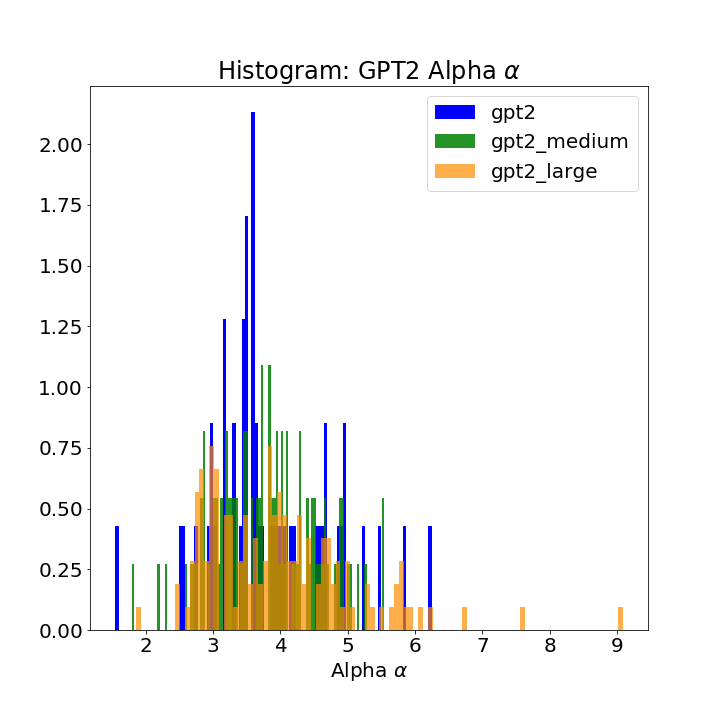
\includegraphics[width=4.5cm]{img/GPT2_all_alpha_hist.png}
        \label{fig:gpt-alpha-layer}
    }
    \qquad
    \subfigure[log Spectral Norm $\log\Vert\mathbf{W}\Vert_{\infty}$]{
        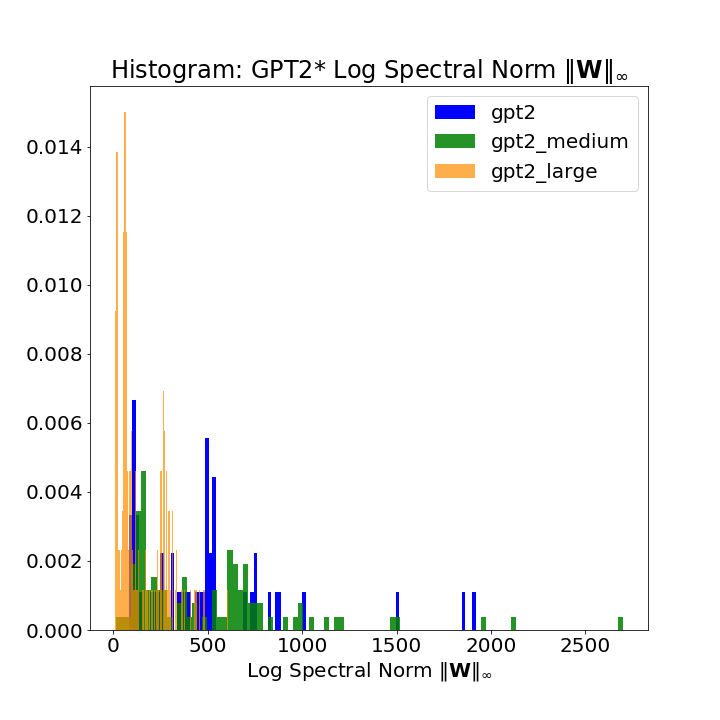
\includegraphics[width=4.5cm]{img/GPT2*_all_spectralnorm_hist.png}
        \label{fig:resnet-snorm-layer}
    }
    \qquad
    \subfigure[log Alpha-Norm $\log\Vert\mathbf{X}\Vert_{\alpha}^{\alpha}$]{
        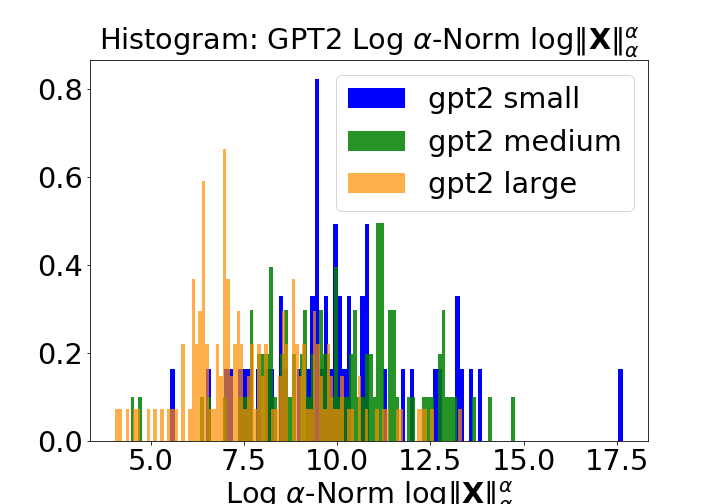
\includegraphics[width=4.5cm]{img/GPT2_all_logpnorm_hist.png}
        \label{fig:gpt-pnorm-layer}
    }
    \caption{Comparison of Power Law Exponnents, Spectral Norm, and Alpha-Norm for different size models in the GPT2 architecture series.  *Note: the log spectral norms (b) histogram omits the first 2 layers, corresponding to the embedding layer, which are normalized differently and have anamolously large values.}
    \label{fig:gpt-alpha-layers}
\end{figure}




